\documentclass{article}

% Language setting
% Replace `english' with e.g. `spanish' to change the document language
\usepackage[english]{babel}

% Set page size and margins
% Replace `letterpaper' with `a4paper' for UK/EU standard size
\usepackage[letterpaper,top=2cm,bottom=2cm,left=3cm,right=3cm,marginparwidth=1.75cm]{geometry}

% Useful packages
\usepackage{amsmath}
\usepackage{graphicx}
\usepackage[colorlinks=true, allcolors=blue]{hyperref}
\usepackage{xcolor}
\usepackage{datetime}
\usepackage[section]{placeins} 
\usepackage{pdfpages}
\usepackage{float}

\title{ME136 Lab 1}
\author{Nathan Yacovetta, Aarchan Saxena, Jobanpreet Mutti, Radhika Marolia}
\date{September 21, 2023}

\begin{document}
\maketitle

\section{Contributions}

\begin{itemize}
\item Nathan Yacovetta: Completed lab tasks and computed the means and standard deviations for section 3b.
\item Aarchan Saxena: Documented Experiment 1.3.1 (motors on and off), added comments to the UserCode, and created the plots for the rate gyroscope outputs for section 3a.
\item Jobanpreet Mutti: Created the plots for the rate gyroscope and accelerometer measurements for both manipulating the vehicle and enabling/disabling noise for sections 3c and 3d.
\item Radhika Marolia: Documented Experiment 1.3.2 (manipulating the vehicle) and formatted/added everything to the lab report on Latex.
\end{itemize}

\section{Running the Motors}

Here is our Usercode.cpp with comments. The code we added is between the capitalized comments "THE CODE THAT WE ADDED STARTS/ENDS HERE" at the bottom of page 1.

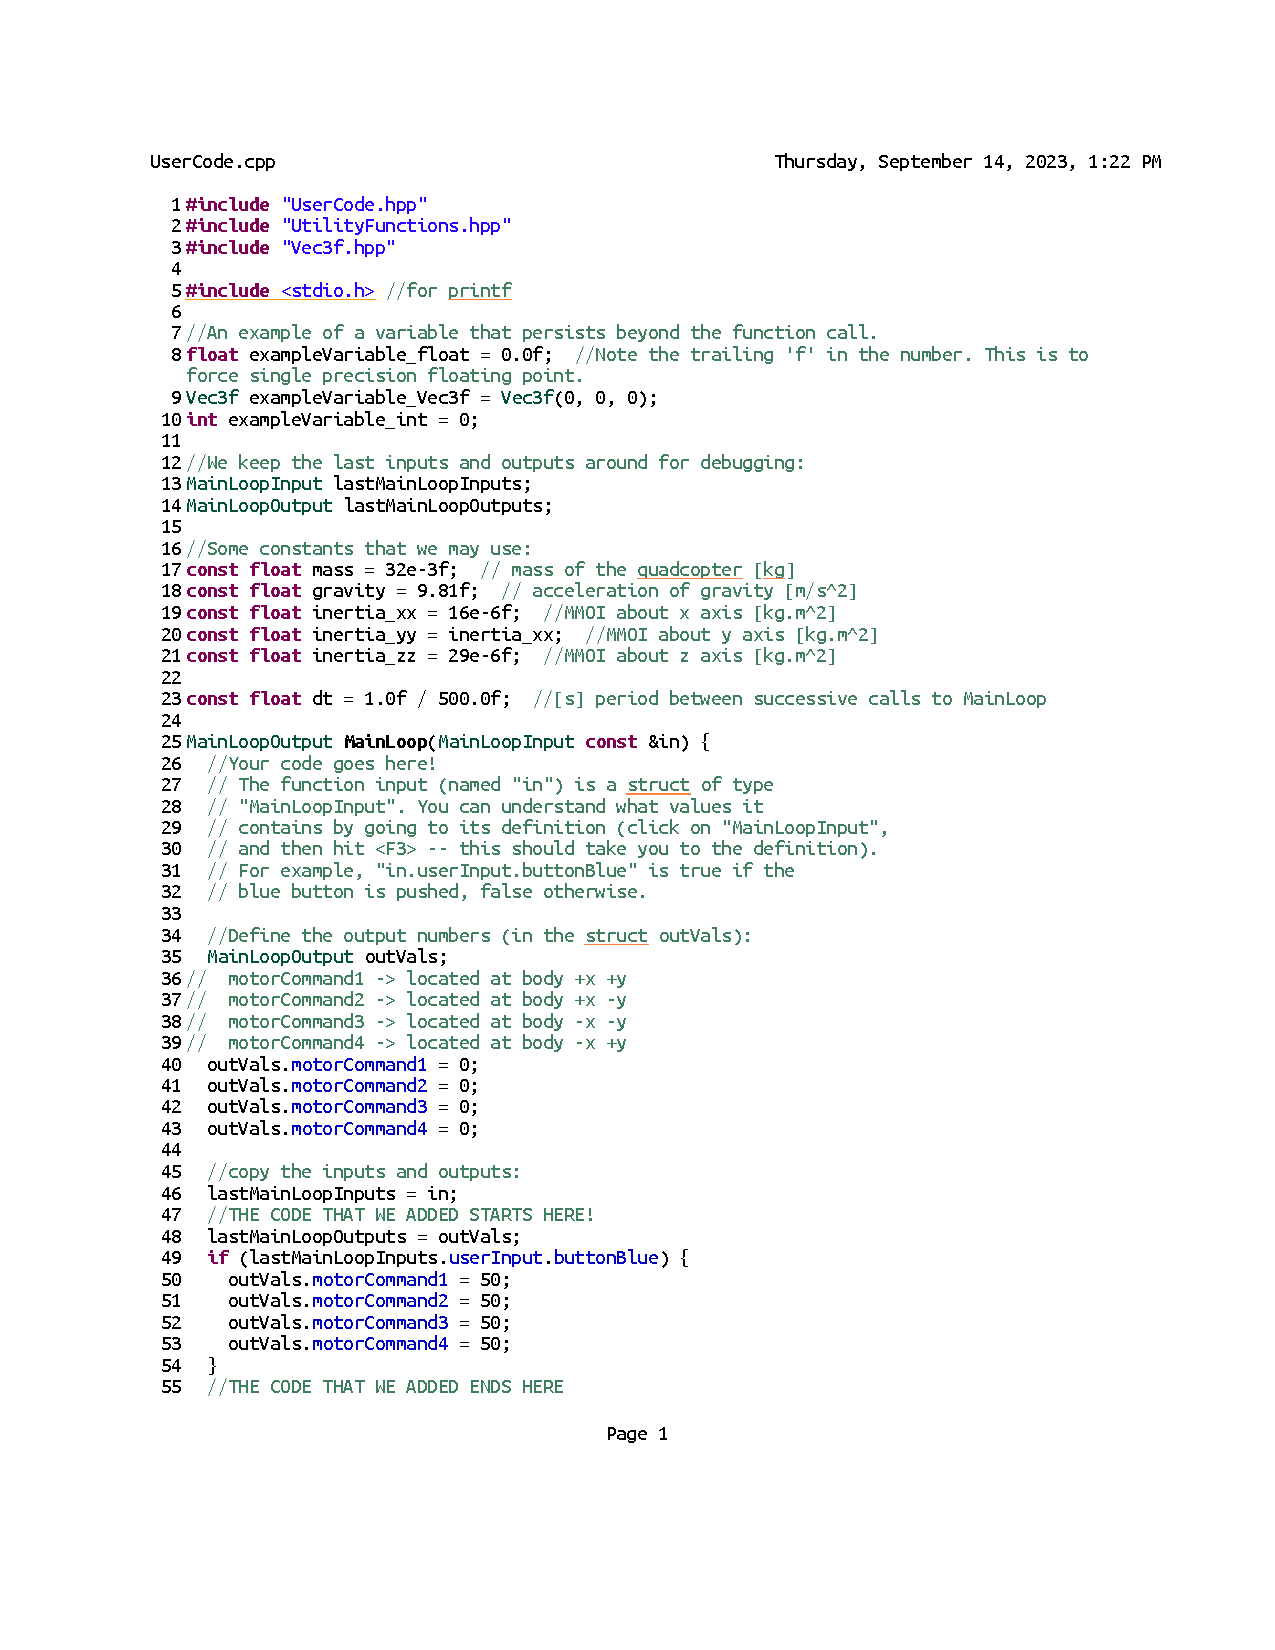
\includepdf[pages=-]{usercode.pdf}

\section{Sensor Analysis}

\subsection {Part A}

\begin{figure}[H]
\centering
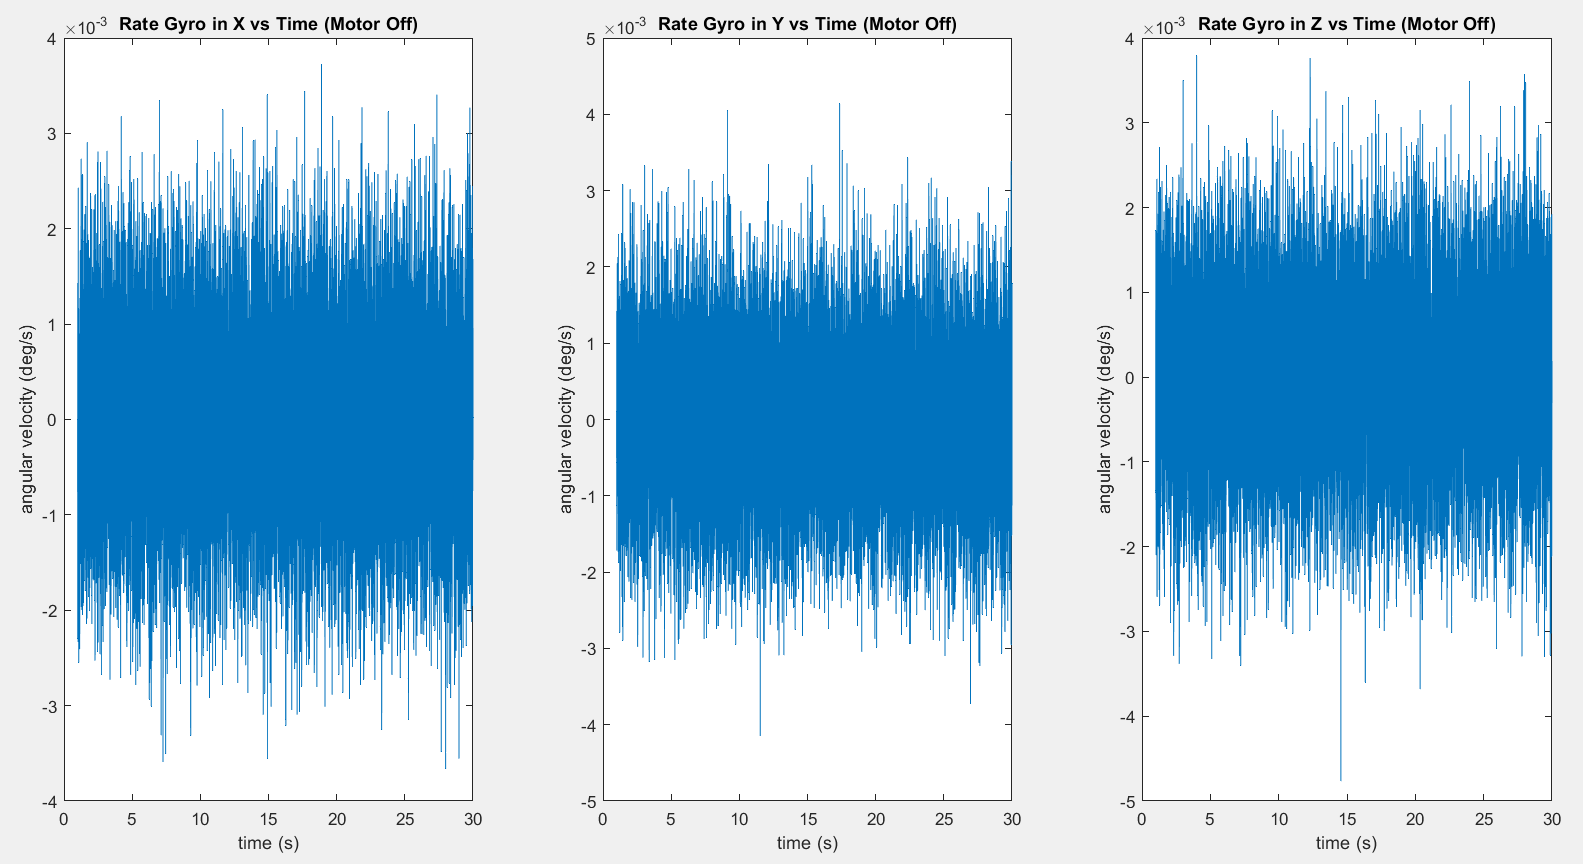
\includegraphics[scale=.35]{me136lab1q3aMotorsOff.png}
\caption{Plot of the Three Rate Gyroscopes with Motors Off \label{fig1}}
\end{figure}
\FloatBarrier

\begin{figure}[H]
\centering
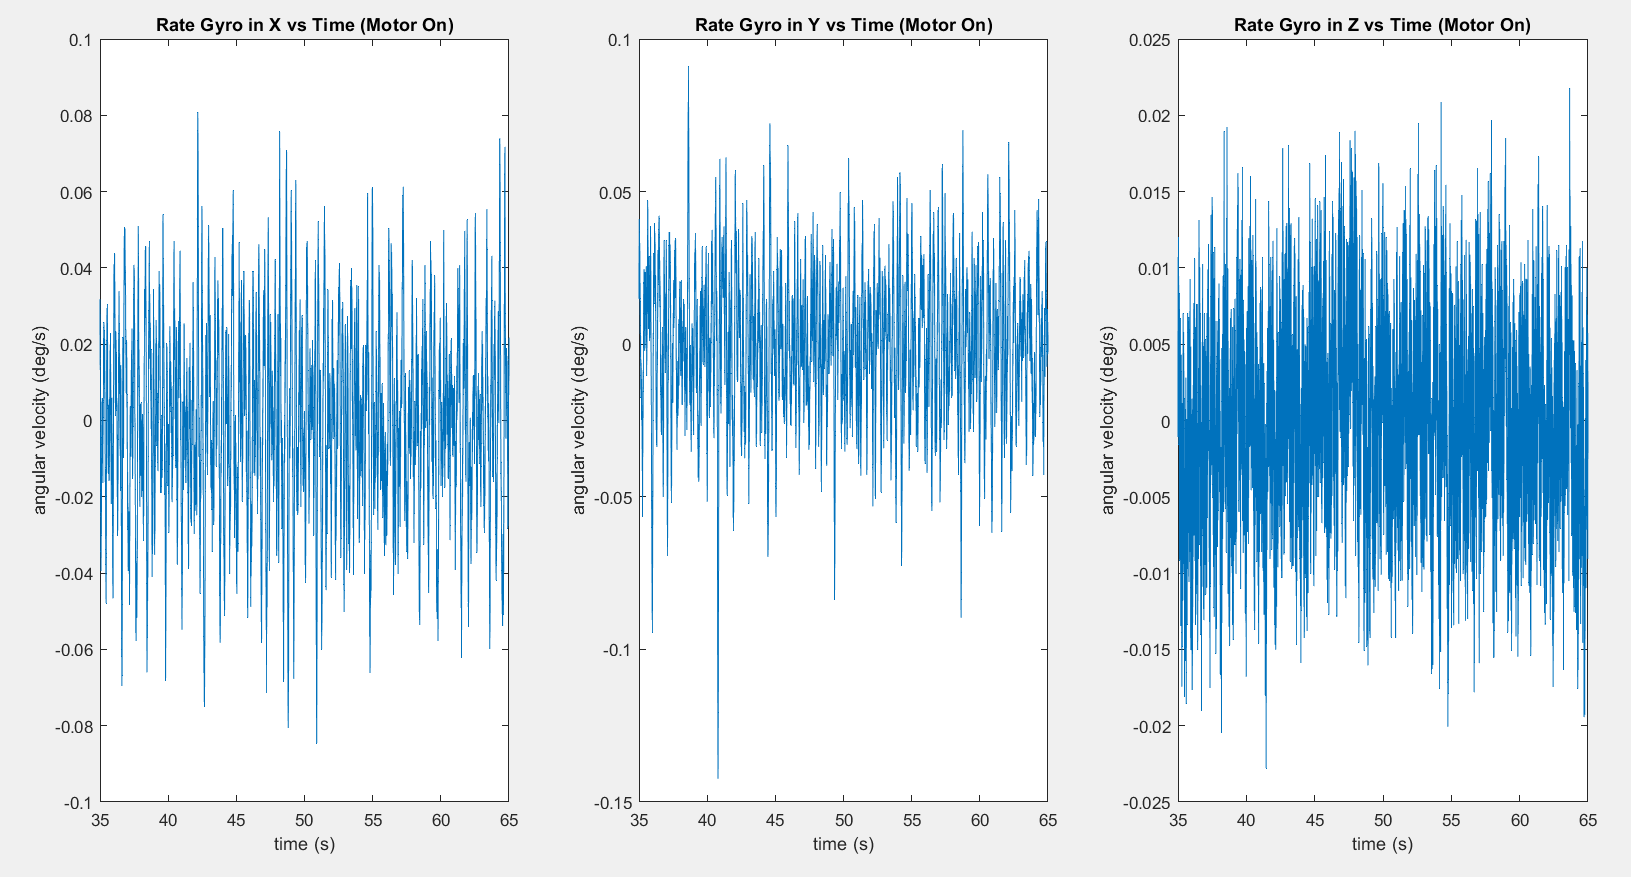
\includegraphics[scale=.35]{me136lab1q3aMotorsOn.png}
\caption{Plot of the Three Rate Gyroscopes with Motors On \label{fig2}}
\end{figure}
\FloatBarrier

\subsection{Part B}

The mean and standard deviations for the rate gyroscope are as follows: 

\begin{itemize}
\item GyroZ(off) mean = -8.5680E-6
\item GyroZ(on) mean = 1.47E-4
\item GyroY(off) mean =  1.1462E-5
\item GyroY(on) mean = -8.8696e-06
\item GyroX(off) mean = 9.7916E-6
\item GyroX(on) mean = 4.4221E-5
\item GyroX (off) STD = 0.0010
\item GyroX (on) STD = 0.0235
\item GyroY (off) STD = 0.0010
\item GyroY (on) STD = 0.0223
\item GyroZ (off) STD = 0.0010
\item GyroZ (on) STD = 0.0054
\end{itemize}

From these results, we can conclude that for both the standard deviation and mean, the value is significantly higher when the drone is on. For the mean, the value is very close to zero. This is expected, as a high value in one direction would imply that the vehicle is turning.

\subsection{Part C}


\begin{figure} [H]
\centering
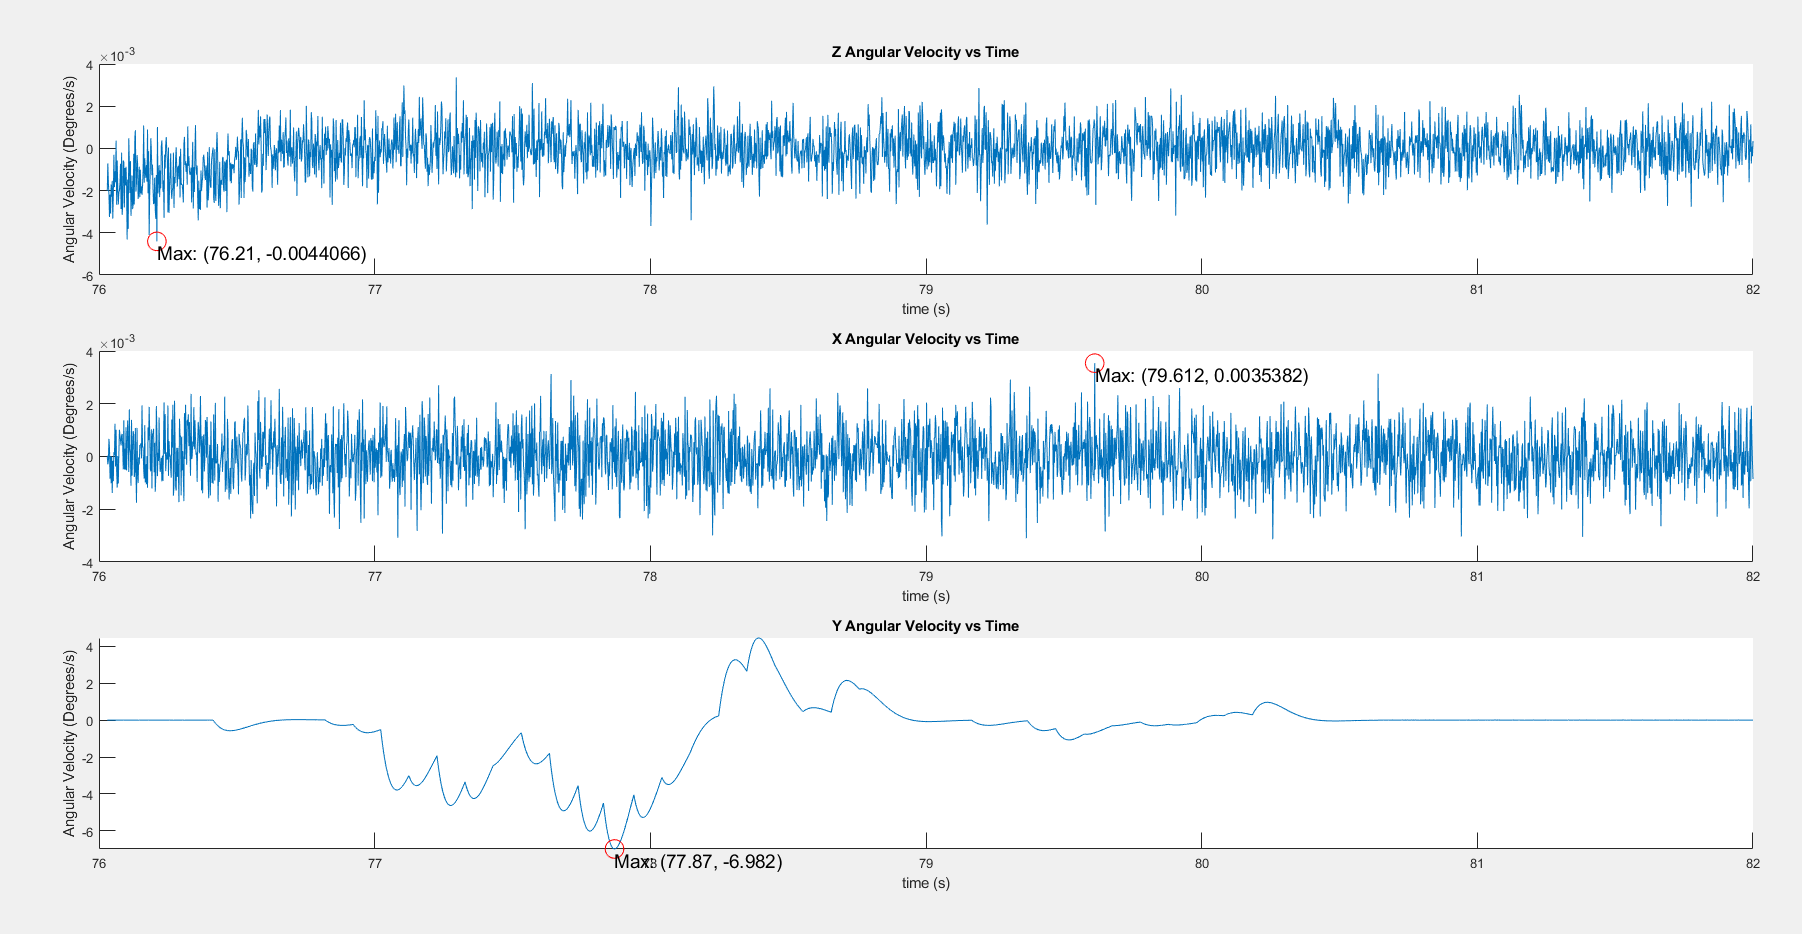
\includegraphics[scale=.32]{me136lab1q3cRateGyroscope.png}
\caption{Three Plots of the Rate Gyroscope when Manipulating the Vehicle \label{fig3}}
\end{figure}
\FloatBarrier

\begin{figure} [H]
\centering
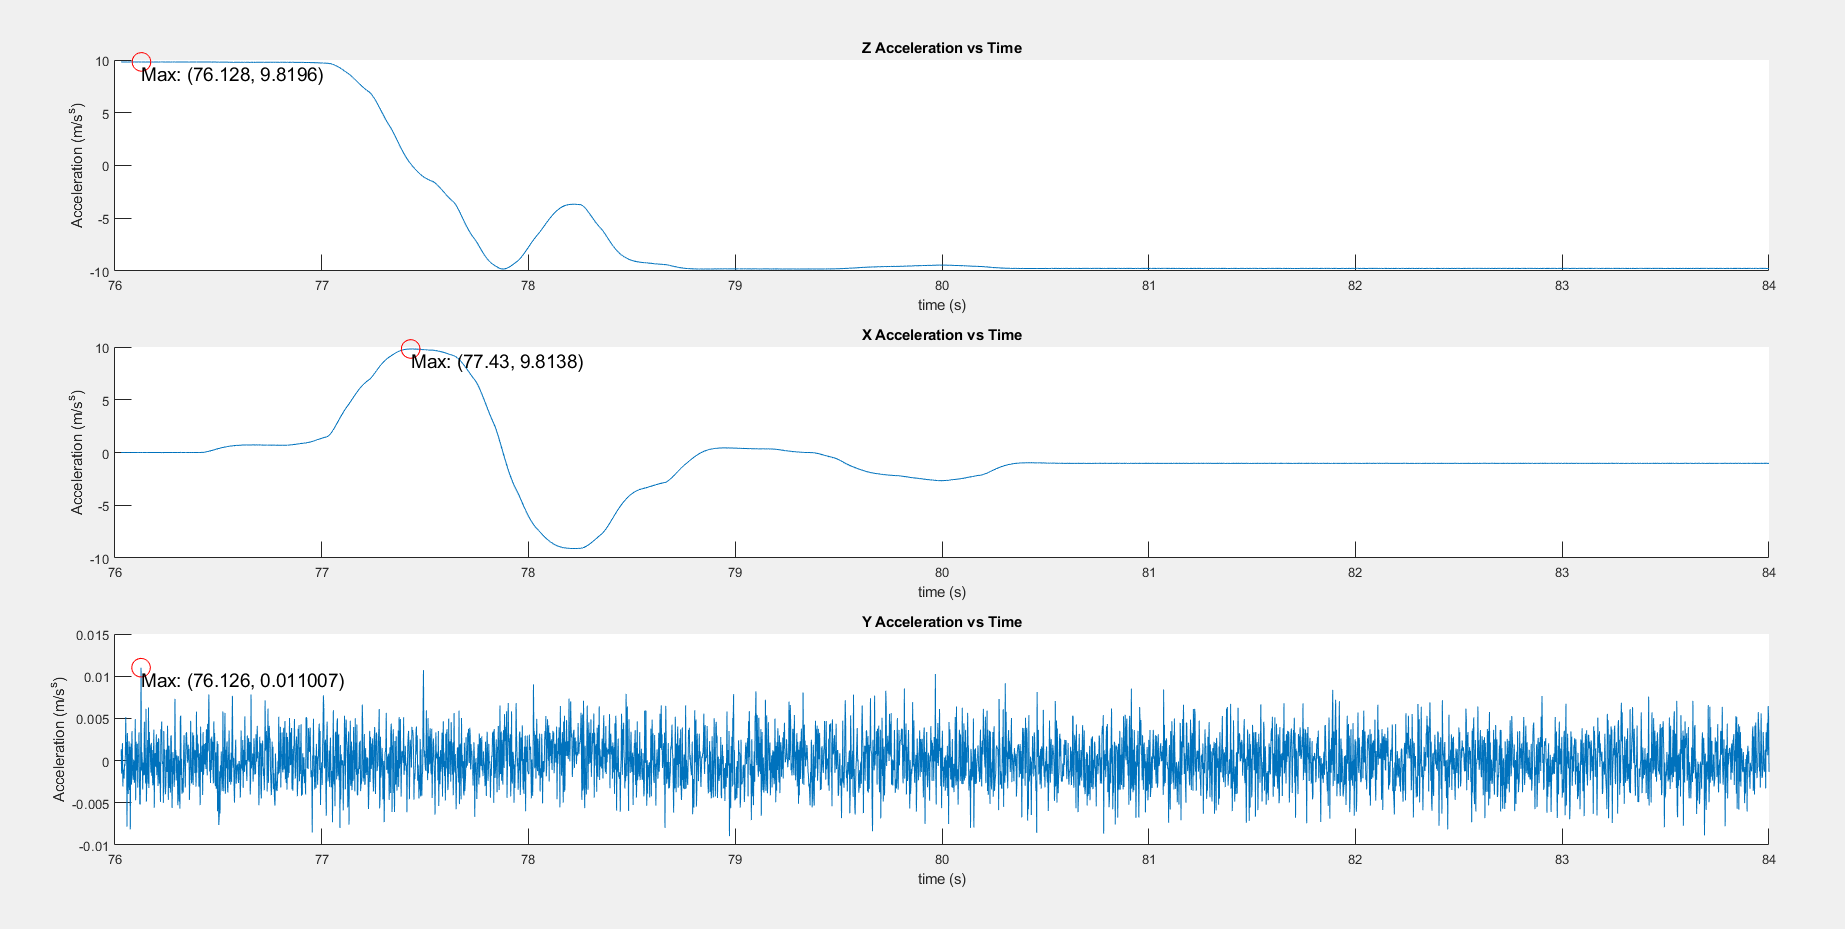
\includegraphics[scale=.30]{me136lab1q3cAccelerometer.png}
\caption{Three Plots of the Accelerometer when Manipulating the Vehicle \label{fig4}}
\end{figure}
\FloatBarrier

From Figure 3, we found that the largest angular velocities are:

\begin{itemize}
\item -0.0044066 $Degrees/sec$ in the z-direction
\item 0.0035382 $Degrees/sec$ in the x-direction
\item -6.982 $Degrees/sec$ in the y-direction
\end{itemize}


From Figure 4, we found that the largest accelerometer measurements are:

\begin{itemize}
\item 9.8196 $m/s^2$ in the z-direction
\item 9.8138 $m/s^2$ in the x-direction
\item 0.011007 $m/s^2$ in the y-direction 
\end{itemize}

These maximum measurements are circled and labeled on their respective plots.






\subsection{Part D}
\begin{figure} [H]
\centering
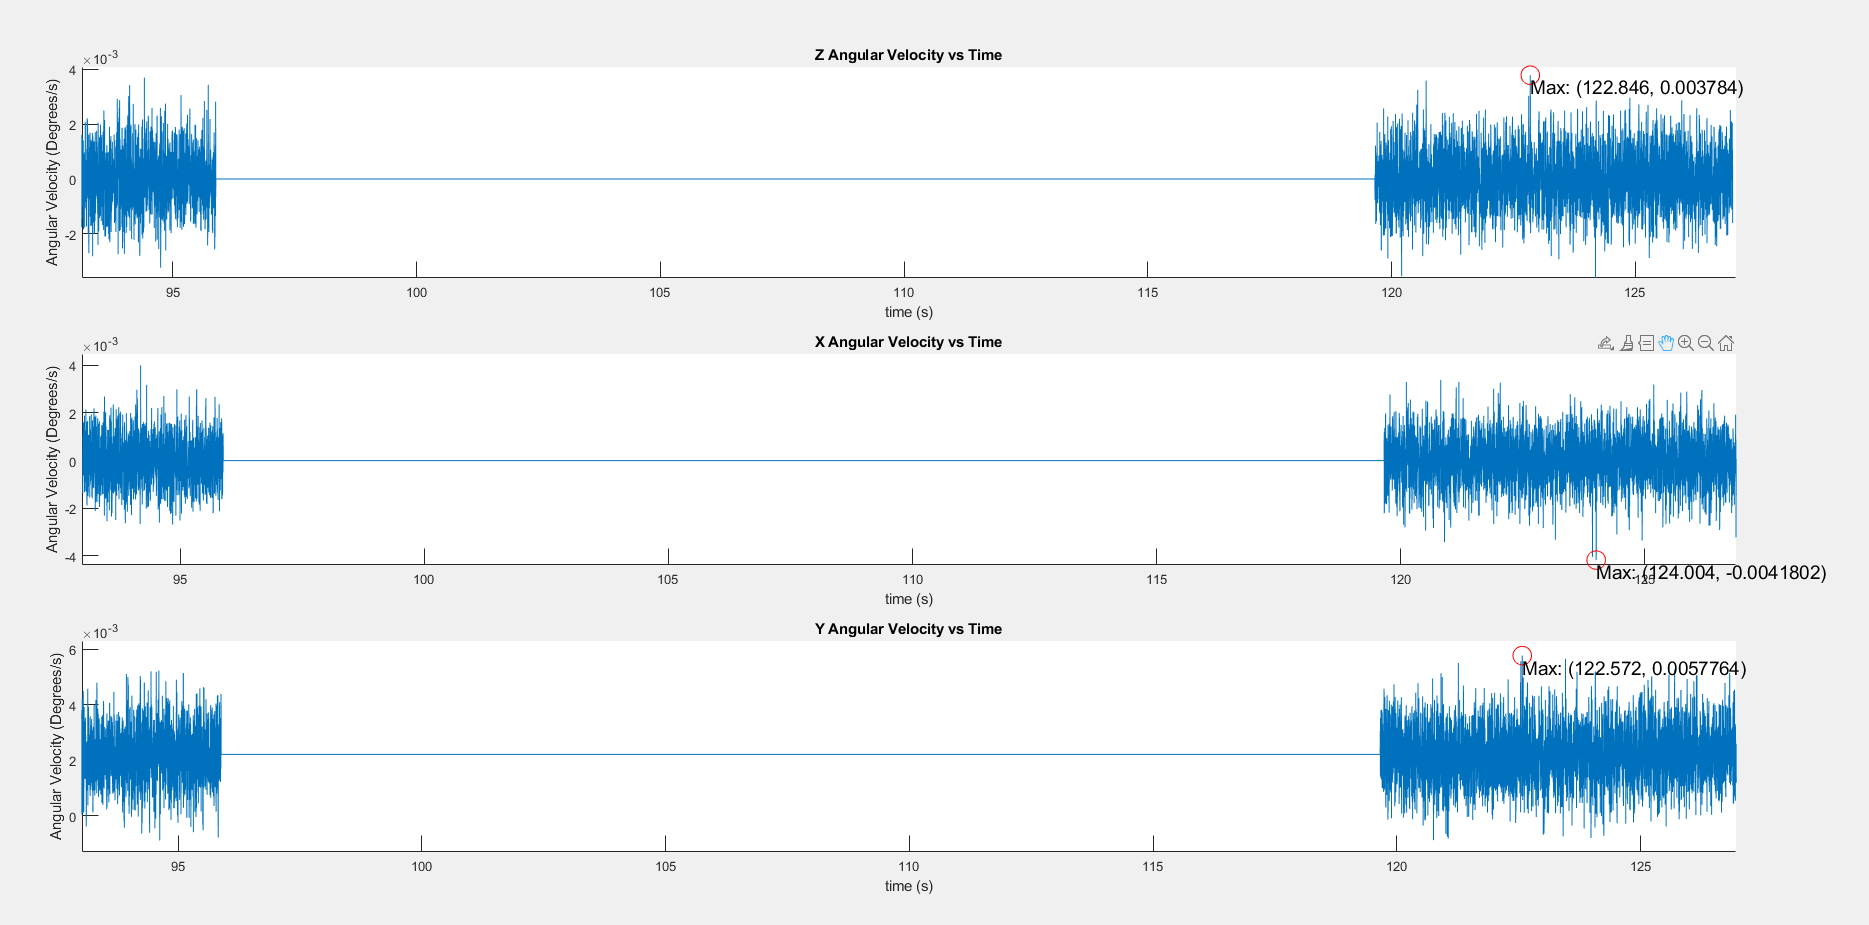
\includegraphics[scale=.30]{me136lab1q3dRateGyroscope.png}
\caption{Three Plots of the Rate Gyroscope with Noise Enabled and Disabled \label{fig5}}
\end{figure}
\FloatBarrier

\begin{figure} [H]
\centering
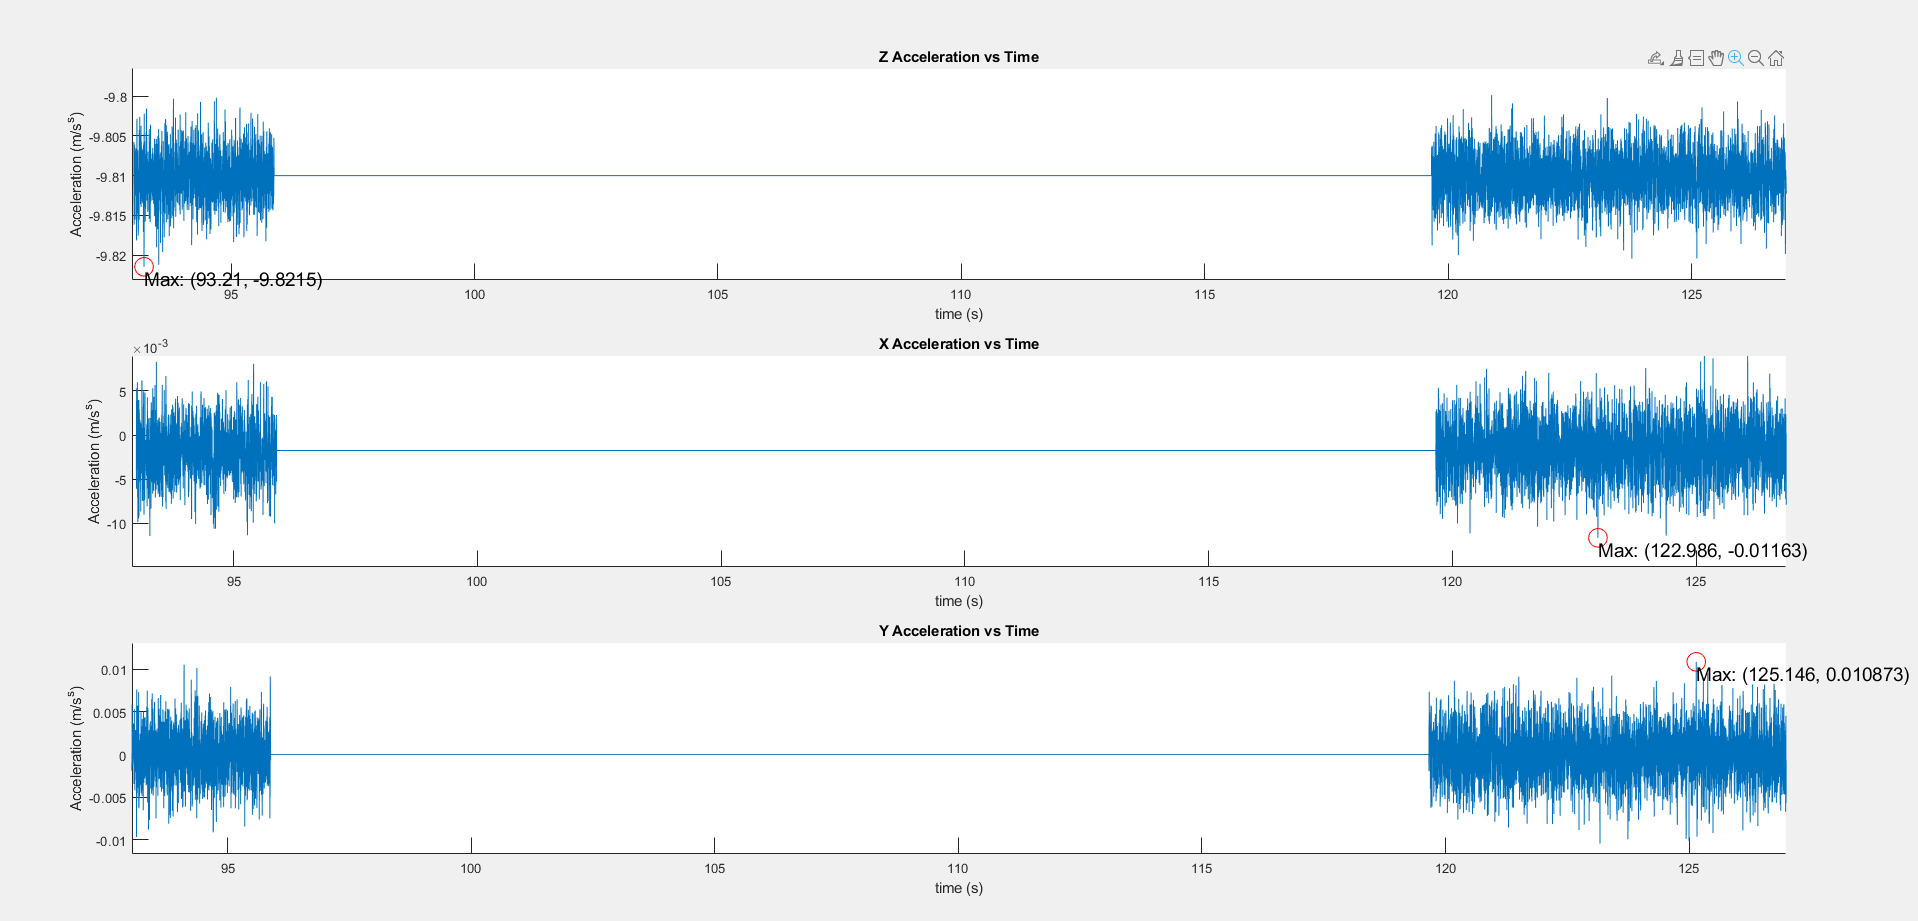
\includegraphics[scale=.30]{me136lab1q3dAccelerometer.png}
\caption{Three Plots of the Accelerometer with Noise Enabled and Disabled \label{fig6}}
\end{figure}
\FloatBarrier

Unlike the graphs from part 3c, these graphs have a section where they are flat. When the noise is disabled in these graphs, the line zeroes out. There are no measurements of angular velocity or acceleration when the noise is disabled. The angular velocity and acceleration graphs are generally very similar.

\subsection{Part E}

To make the plots, we used Matlab. We chose Matlab because all of the members in our group are much more comfortable using the array features in Matlab over python.

\end{document}